\chapter{Regra de Três Simples e Composta}

\section{Regra de Três Composta}

\quest{Oficial de Justiça 2023 - VUNESP}
{Considere as informações apresentadas na tabela a seguir, relacionadas à produção de certa peça que é
realizada apenas por máquinas iguais, trabalhando ao mesmo tempo, com a mesma capacidade de produção.\\
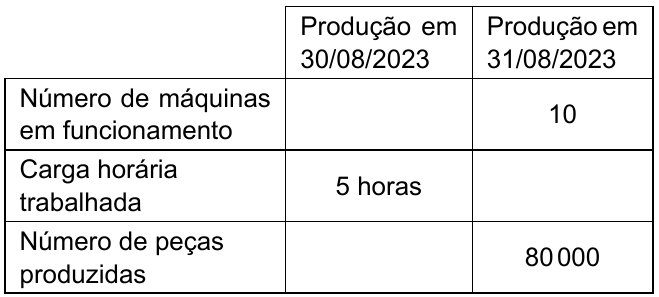
\includegraphics[scale=.5]{fig002.png}\\
Sabendo-se que as informações apresentadas são proporcionais, que em 30/08/2023 o número de máquinas
em funcionamento era um quinto maior que o número de máquinas trabalhando no dia seguinte, e que o número
de peças produzidas em 31/08/2023 foi quatro terços do número de peças produzidas no dia anterior, é correto afirmar que a carga horária trabalhada no dia 31/08/2023 foi de}
{\item 8 horas.
\item 7 horas.
\item 9 horas.
\item 8 horas e 30 minutos.
\item 7 horas e 30 minutos.}
{https://youtu.be/mVp0Bf8s8J4}

\quest{Banco do Brasil 2023 - CESGRANRIO}{G máquinas idênticas imprimem G panfletos idênticos, em G dias, trabalhando G horas por dia. H máquinas idênticas às primeiras imprimem H panfletos idênticos aos primeiros, em T dias, trabalhando H horas por dia. Portanto, T é igual a
}{\item $\dfrac{H^2}{G}$
\item $\dfrac{G^3}{H}$
\item $\dfrac{H^3}{G^2}$
\item $\dfrac{G^2}{H}$
\item $\dfrac{G^2}{H^3}$ }{https://youtu.be/3GMewuLWYz0}
